%% ma: L12-B13-0037
%% lop: 12
%% chuong: 4
%% bai: 13
%% dang: 12.13.2
%% loai: TN4
%% muc: TH
%% dap_an: "D"
%% nguon: "(NBV)-ĐỀ SỐ 18-MỖI NGÀY 1 ĐỀ THI 2025.pdf (D18, MỖI NGÀY 1 ĐỀ - Đề số 18), Phần I Câu 8"
%% kien_thuc: "Bài 13 (thể tích vật thể theo diện tích thiết diện S(x))"
%% trang_thai: chinh-thuc
%% ghi_chu: "Đáp án gốc D đúng (S(x) = 9 - x^2, V = 18). Trùng ý tưởng với dạng đã duyệt 12.13.2 (thể tích vật thể qua diện tích thiết diện), nhập chính thức. Đề gốc in phương án A là 171π và B là 171 (giữ nguyên, hai phương án nhiễu). Hình dựng lại: vật thể đặt trên đáy là một phần tư hình tròn bán kính 3 (mặt phẳng Oxy), thiết diện hình vuông đứng vuông góc trục Ox; hình gốc vẽ khối hộp minh họa nên chỉ mang tính tượng trưng."
\begin{ex}
Khi cắt vật thể bởi mặt phẳng vuông góc với trục $Ox$ tại điểm có hoành độ $x$ $(0\le x\le3)$ ta được mặt cắt là một hình vuông có cạnh là $\sqrt{9-x^2}$ (được mô hình hóa bởi hình vẽ bên dưới). Thể tích của vật thể đó bằng
\begin{center}
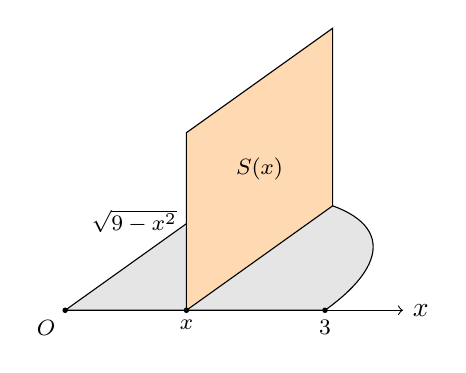
\begin{tikzpicture}[x={(1.1cm,0cm)},y={(.7cm,.5cm)},z={(0cm,.85cm)}]
  \def\xo{1.4}
  \pgfmathsetmacro\so{sqrt(9-\xo*\xo)}
  \fill[gray!20] (0,0,0)--(3,0,0)--plot[domain=0:90,variable=\t,samples=40]({3*cos(\t)},{3*sin(\t)},0)--cycle;
  \draw (0,3,0)--(0,0,0)--(3,0,0)--plot[domain=0:90,variable=\t,samples=40]({3*cos(\t)},{3*sin(\t)},0);
  \fill[orange!30] (\xo,0,0)--(\xo,\so,0)--(\xo,\so,\so)--(\xo,0,\so)--cycle;
  \draw (\xo,0,0)--(\xo,\so,0)--(\xo,\so,\so)--(\xo,0,\so)--cycle;
  \draw[->] (3,0,0)--(3.9,0,0) node[right]{$x$};
  \fill (0,0,0) circle (1pt) (3,0,0) circle (1pt) (\xo,0,0) circle (1pt);
  \path (0,0,0) node[below left,font=\footnotesize]{$O$} (3,0,0) node[below,font=\footnotesize]{$3$}
        (\xo,0,0) node[below,font=\footnotesize]{$x$}
        (\xo,{\so/2},{\so/2}) node[font=\footnotesize]{$S(x)$}
        (\xo,0,{\so/2}) node[left,font=\footnotesize]{$\sqrt{9-x^2}$};
\end{tikzpicture}
\end{center}
\choice{$171\pi$}{$171$}{$18\pi$}{\True $18$}
\loigiai{Diện tích mặt cắt là $S(x)=\left(\sqrt{9-x^2}\right)^2=9-x^2$. Thể tích vật thể là
\[V=\int_0^3S(x)\,\mathrm dx=\int_0^3(9-x^2)\,\mathrm dx=\left(9x-\dfrac{x^3}3\right)\Big|_0^3=27-9=18.\]
Chọn D.}
\end{ex}
